\documentclass[]{article}
\usepackage{xcolor}
\usepackage{mdframed}
\usepackage{graphicx} 
\usepackage{mcode}
\usepackage{fontawesome}
\usepackage{amsmath}
\usepackage{hyperref} 
\usepackage{xcolor}

% your names and student id's go here: 
\newcommand{\StudentA}{First Student}
\newcommand{\StudentB}{Second Student}
\newcommand{\StudentIdA}{1234567890}
\newcommand{\StudentIdB}{0987654321}

\newcommand{\dueDate}{4.1.2016}

\newcommand \BeginAnswer {\begin{mdframed}[backgroundcolor=blue!15]} 
\newcommand{\EndAnswer}{\end{mdframed}}
\renewcommand\thesection{Part \Alph{section}-}
\renewcommand\thesubsection{\arabic{subsection}.}
\renewcommand\thesubsubsection{\thesubsection\arabic{subsubsection}}  
\newcommand{\code}{\item[\faKeyboardO]}
\newcommand{\quest}{\item[\faPencil]}

% Title Page
\title{Sparse Representations and Their Applications in Signal and Image Processing \break\\
	 Home Work 2: Iterative Shrinkage Algorithms}

\author{Submitted by: \begin{tabular}{cc}
		\StudentA & \StudentIdA \\ 
		\StudentB  & \StudentIdB 
	\end{tabular}}
\date{due \dueDate}

\begin{document}
\maketitle
\section*{Instructions} 
 
\begin{itemize}
	\item Work should be done in pairs and submitted via moodle. Students wishing to submit on their own need to get permission to do so in advance. 
	\item Submission should include a pdf-file containing the report and all Matlab files you created for this exercise.
	\item You are encouraged (but not obligated) to use \LaTeX\ for your report, and add your answers to the project \texttt{.tex} file that is included with the exercise files. \emph{You will get a 5 point bonus for doing so. However, the maximal grade will be 100 in any case for the exercise}.
	\item The items that require you to code or write an answer have an icon of keyboard or pen respectively.
	\BeginAnswer
	If you decide to submit your file in LaTeX, make sure your answers and figures are placed inside a 
	\texttt{\textbackslash BeginAnswer} \ldots \texttt{\textbackslash EndAnswer} 
	block that places what you added in a box such as this one.
	\EndAnswer 
	\item Write your own code. This exercise is meant to teach you how the different algorithms operate.
	\item Indent and highlight the Matlab code you attach to the report. In LaTeX this is done using the command: \lstinline|\lstinputlisting{<filename>}| from the package \lstinline|mcode.sty|, which is already included in the homework laTeX file. 
	\item Use sparse type vectors and matrices in your code when it is appropriate.
	\item Questions regarding the exercise should be asked in the course forum in moodle, e-mails about the exercises will not be answered.    
\end{itemize}

\section{ Synthetic Data Generation} 
The goal of this exercise is to get you acquainted with the various algorithms and to measure their performance. Throughout the assignment, you will be seeking to minimize the following expression:
\begin{equation}
f(x) =  {1\over 2}\|y-CDx\|^2_2 +\lambda \|x\|_1 \label{eq1}
\end{equation} 

Here $y$ represents an image and $x$ is its representation using the dictionary $D$. Our dictionary is going to be the 2-D  Haar basis (inverse of the 2-D Haar transform, which is simply the transpose of the Haar transform as the Haar wavelet is unitary). 
We will use the following convention: $Y_0$ is an $s\times s$ image we wish to recover and $y_0=\text{vec}(Y_0)$ is its column stack representation. The 2-D Harr transform coefficients are $X = \text{haar2D}(Y_0)$ ($s\times s$ matrix), and $x=\text{vec}(X)$ is its column stack vector. We are presented with a corrupted measurement $y$, which is related to $x$ using the relationship $y=CDx+n$, where $n$ is a noise vector, $D$ represents the inverse of the Haar transform and $C$ is a sampling matrix.  

\subsection{Dictionary - $D$ }
\begin{itemize}
	\item Set $s=128$ and define $D$ to be the $128^2\times 128^2$ matrix representing the 2-D Haar basis in \emph{vector} form (hence the $s^2$ size). \emph{At this point you need to start using the} \lstinline|sparse| \emph{matlab function}   
	
	
\end{itemize} 

\subsection{Sampling Matrix - $C$} 
We will be experimenting with three types of sampling matrices, defined using a parameter $p$ that stands for the 'compression' or amount of omitted pixels. The size is going to be $m\times n$ where $n=s^2$ is the dimension of the unknown signal $x$ (remember $D$ is square) and $m=\lfloor ps^2\rfloor$ is the amount of measurements we receive.        
\begin{enumerate}
	\item $C_d$ of size $m\times n =\lfloor ps^2\rfloor\times s^2$ represents deletion of pixels from an image. Generate this matrix by deleting $n-m$ random rows from the identity matrix of size $s^2 \times s^2$, {\color{blue} and then multiply it by an averaging filter of size $l$, e.g. as follows:  }
	\begin{lstlisting}
	 l = 2;    
	 v = [ones(1,l) / l, zeros(1,s-l)];  
	 M = sparse(toeplitz(v,v)); 
	 C_a = kron(M,M); 
	 C_d = eye(n);
	 C_d = C_d(sort(randperm(n,m)),:);
	 C_d = sparse(C_d*C_a); 
	      
	\end{lstlisting}
	
	\textbf{After $C_d$ is generated check to see that none of the atoms in $D$ are zeroed entirely when multiplied by $C_d$. if that happens, regenerate the matrix, {\color{blue} if the problem persists enlarge $l$}. }
	
	\item $C_g$ is a Gaussian sampling matrix (known also as a sensing matrix) of size $m\times n =\lfloor ps^2\rfloor\times s^2$, with i.i.d. entries drawn uniformly at random from $\mathcal{N}(0,1)$
	
	\item $C_b$ of size $n\times n$, which represents a 11-tap Gaussian blur kernel. Use the following code snippet to generate it: 
	\begin{lstlisting}
	     %Half of an 11 tap Gaussian filter:  
	     v = exp(-0.5*(0:5).^2); 
	     %Normalize:
	     v = v/(v(1) + 2*sum(v(2:end))); 
	     %Create the 1-D filter matrix of size sxs:  
	     M = sparse(toeplitz([v, zeros(1,s-numel(v))],[v, zeros(1,s-numel(v))])); 
	     %Create the 2-D vector form blur operator:
	     C_b = kron(M,M);
	\end{lstlisting}
	 
\end{enumerate}
\emph{Write your code in such a way that the multiplication $CD$ is never calculated nor stored, i.e. your code contains only vector and matrix operations.}

\subsection{Measurement $y$ and the Unknown $x$ }  
\begin{itemize}
	\item Generate the set $T$ of size $k$ (e.g. $k=30$) from the set $\{1\ldots n\}$ (without repetitions). This is going to be the 'true' support. Use the following code snippet: 
	\begin{lstlisting}
	T = randperm((s/4)*(s/4+1),min(ceil(k/2),40)); 
	T = mod(T,s/4) + s*(floor(T/(s/4)));
	while length(T) < k 
	T = unique([T, randperm(n,k-length(T))]);
	end
	\end{lstlisting}
	\item Generate $x$, the unknown parameter, such that $x_i \sim \mathcal{N}(0,1),\ i\in T$; $x_i=0,\ i \notin T$.  
	\item Generate $y_0=Dx$ that represents the clean, uncompressed signal. 
	\item Generate $y = Cy_0+w$ where $w$ is an i.i.d. Gaussian white noise vector of appropriate length with variance $\sigma^2_n$. This time set $\sigma_n$\lstinline|(=sig_n)=dr_ratio*dr|,  where $dr = max(Cy_0) - min(Cy_0)$, and \lstinline|dr_ratio| is an input to the function \lstinline|GenData| (see below).  
\end{itemize}
\subsection {Wrapping Function} 
\begin{itemize} 
	\code Write the function \\
	\lstinline|[C_g, C_d, C_b, D, T, x, y_d, y_g, y_b, y0]=GenData(p,k,dr_ratio)|.    
	\item 	Below you can see an example for \lstinline|p|=20\% and \lstinline|dr_ratio| = 2\%. The figures are the matrix form of the vectors: 
	\begin{itemize}
		\item original: $y_0$  
		\item deletion: $C_d^Ty_d = C_d^T(C_dy_0+w)$ 
		\item blur: $y_b = C_by_0+w$ 
		\item compressed sensing: $C_g^\dagger y_g= C_g^\dagger (C_g y_0 + w) $. 
	\end{itemize}
	\centering{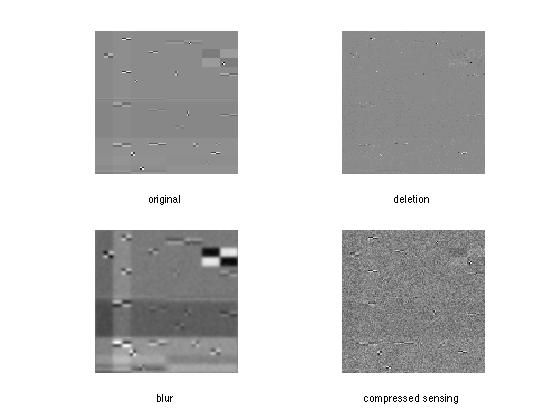
\includegraphics[width=.7\linewidth]{figs/data}}

\end{itemize}

\section { Initial Results  }
\label{sec:init}
Let us compare some straight-forward solutions to our problem of recovering $x$ from $y$ in \eqref{eq1}. Our tools for comparison will be the following: 
\begin{enumerate}
	\item  $PSNR(y_0,\hat{y}) = db(s^2\cdot dr^2 / \|y_0-\hat{y}\|_2^2) $, where $dr=max(y_0) - min(y_0)$ is the dynamic range, and $db(\cdot) = 10\log_{10}(\cdot)$.   
	\item $SSIM(Y_0,\hat{Y})$ - Structured Similarity Index Measure, can be calculated by the matlab function of the same name. 
	\item $MSE(x,\hat{x})=\|x-\hat{x}\|^2_2 / \|x\|^2_2$ - Mean Squared Error in $x$.
\end{enumerate}

Above, $\hat Y$ represents the reconstructed image of size $s\times s$ and $\hat x$ is its estimated coefficients. More specifically $\hat Y$ is $\hat y$ rearranged as an image and $\hat y = D\hat x $  .  


Use the following estimators for $\hat{y}$: 
\begin{enumerate}
	\item Oracle - Calculate the image that minimizes $\|y-CDx\|_2$ given that the \textbf{true support $T$ is known}. \emph{In reality we don't have access to this information, but under certain conditions some methods can achieve 'oracle' or 'near oracle' performance making the oracle estimator a good tool for comparison}
	\item $L_2$-estimator - compute the image that solves the following optimization problem: 
	$$ \hat{y} = D\hat{x}, \ \ \ \ \ \hat{x} = \min_{\hat{x}} \|\hat{x}\|^2_2 \ \ s.t.\ \ y = CD\hat{x}   $$
	\textbf{Do this by running the conjugate gradient method (google it) for at least 500 iterations, and remember to use only vector-matrix multiplications (i.e. no multiplying $C$ and $D$ directly)  }
	\code Write the file \lstinline|PartB.m| that evaluates the performance of the oracle and $L_2$ estimators. Present the results in a clear way and calculate the $PSNR$, $SSIM$ and $MSE$ of each method. Present the resulting images alongside the original $y_0$ you generated. \textbf{Pick a value (as you wish) for \lstinline|dr_ratio| from the range 1\%-3\%, for \lstinline|p| from the range 10\%-30\% and for \lstinline|k| from  the range 30-60. Do not change these values for the remainder of the exercise (bar the last part)}  
	\quest Discuss the results and try to explain the performance you get.
	
\end{enumerate} 


\section{ Shrinkage Algorithms} 
\subsection{Implementation}
 Implement the following algorithms. You might need to visit Wikipedia and chapter 6 in the course book \cite{mikibook} (or use other sources if you wish) to learn more on some of the subjects mentioned.
\begin{itemize}
	\code \lstinline|ista| - Iterative Shrinkage Thresholding Algorithm \cite[fig. 6.1]{mikibook}.
	\code \lstinline|ista_ls| - ISTA with a a line search - \cite[p. 127]{mikibook}, using the armijo rule (Google it).   
	\code \lstinline|fista| - FISTA with a constant step size \cite[section 4]{beck2009fast}
\end{itemize}
\emph{Implementation notes:} 
\begin{itemize}
	\item Initialize all algorithms with $\hat x = 0 $.  
	\item Use the following $f$: \begin{equation}
\lstinline|f = @(x) lambda * norm(x,1) + 0.5 * norm(y - C*(D*x),2)^2| \label{eq:f} 
	\end{equation}
	\item Calculate and store the value of $f$ and the PSNR at each iteration of the algorithms. Plot these quantities ($f$ and PSNR as function of the iteration number) along with the algorithms' final output.  
	\item There is no need to normalize the columns of $CD$ to unit norm. You can do this if you want but if you decide to do that be careful to do it efficiently.    
	\item The algorithms should get both $C$ and $D$ as their input. 
	\item You should implement two stopping criteria for your algorithms: (i) difference between subsequent estimates is small (i.e., $\|\hat x_{i+1} - \hat x_i\|_2^2 \leq \epsilon_t$ for some small constant $\epsilon_t$, where $i$ is the iteration number); and (ii) a limit on the maximal amount of iterations the algorithm can run. The algorithm should stop if one of these criteria is met.   
	\item \emph{Advice:} when debugging your implementation, you might want to set $s$ to be smaller than $128$, so the code will run faster. 
\end{itemize}



\subsection{Testing}
\begin{itemize}
	\code Create the file \lstinline|PartC.m| to hold the code for the tests you perform in this section.
	\item Work in this fashion: 
	\begin{enumerate}
		\item Find the maximal eigen-value ($\lambda_{\max}$, a.k.a. the matrix norm) of $D^TC^TCD$ using the power method (google it), and set $c = \lambda_{\max}$ in ISTA.
		\item Use ISTA to seek for a good value of $\lambda$ that yields a good PSNR and a sufficiently sparse solution (with less than $10\cdot k$ non-zeros). The limit of the number of ISTA iterations in this step for every candidate value of $\lambda$ should be at least 1000. 
		\item Run all three algorithms with the $\lambda$ you found until convergence is reached or the limit on the number of iterations is met.  
		\item Use debiasing after you get a solution, similar to the LARS part of the previous homework assignment. You may want to use the conjugate gradient algorithm to solve the least squares problem you get in the debiasing step.    
	\end{enumerate} 
	\item Plot a graph of the value of $f$ and the PSNR as a function of the iterations for each of the methods and the three types of sensing matrices. 
	\quest Is the PSNR monotonically decreasing? \emph{Hint: there are papers that deal with this issue, e.g. \cite{giryes2011projected}}. 
	\code Compare the resulting SSIM, MSE, PSNR, and the sparsity of the obtained solution for each of the methods. Present the resulting images. 
	\quest Compare the MSE and PSNR before and after debiasing, did it improve? by how much?   
	\quest Discuss the results: Which method is better and when? What are your conclusions? 
\end{itemize}

\section{De-Blurring and Inpainting of a Real World Image}
We will now try to de-blur and inpaint a real world image. Often this is done using redundent dictionaries (unlike the square orthogonal dictionary used in this exercise). An example for such a redundent dictionary is the undecimated Haar transform (see for example the deblurring  examples in \cite{beck2009fast} and \cite{giryes2011projected} for more details). Here, we will settle with the orthogonal Haar that you have already generated.   
\begin{itemize}
	\code Create the file \lstinline|PartD.m|
	\item Set: 
\begin{lstlisting}
Y0 = double(rgb2gray(imread('cameraman.jpg')));
Y0 = Y0 / max(Y0(:));
\end{lstlisting}
The file \lstinline|cameraman.jpg| is supplied with the exercise files.
\code Plot the energy in the coefficients $x_0$ sorted in descending order. 
\quest Is the sparsity assumption valid for this image? Explain.   
\item Repeat the experiments in Part B. {\color{blue} using only $C_d$ (dont forget to apply the averaging filter before deleting pixes, as explained above) with $p=0.5$ and $dr=1\%$} . For the oracle estimator support choose a few thousands of the largest coefficients (in absolute value) of $x_0$ in the Haar basis. {\color{blue} See the following figure for how the original and the generated image should look like:} 

{\centering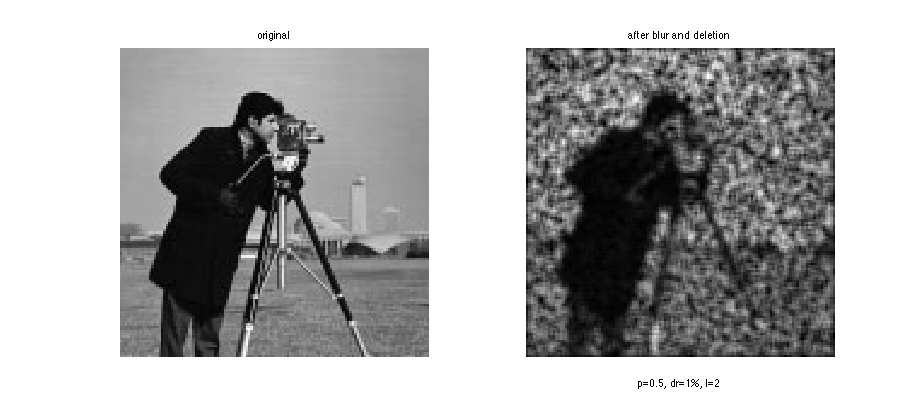
\includegraphics[width=\linewidth]{figs/cm}}


\item Now run the algorithms from Part C. {\color{blue} Try to achieve a solution with  $\sim 4000-5000$ non zeros} 
\quest Explain the role of $\lambda$ in the output result. What will happen if $\lambda$ is too small? What will happen if it is too large? 
\quest {\color{blue} Did debiasing help in this case?} 
\quest Present and discuss the results you get. 
\code Bonus challenge: try to de-blur an image of your own (of size 128$\times$ 128). 
\end{itemize}
\section*{Wrap Up}
\begin{itemize}
	\code Create the file \lstinline|RunMe.m| that can be used to run all the code for this exercise and recreate your results 
	\item Submission in moodle should include two files: 
	\begin{itemize}
		\item Your report in PDF format, named \lstinline|SparseRepHw2_<student #1>_<student #2>.pdf|.
		\item Compressed ZIP file named \lstinline|SparseRepHw2_<student #1>_<student #2>.zip| containing your report and matlab code.  
	\end{itemize}   
\end{itemize}

\bibliographystyle{plain}
{\bibliography{hw_refs}}
\end{document}          
